\chapter{Champs scalaires}
%
Un champ scalaire est une {\it application} qui associe à chaque {\it point de l'espace-temps} un {\it scalaire} (un nombre).

Dans ce chapitre, nous présentons deux exemples de champs scalaires.


%%%%%%%%%%%%%%%%%%%%%
\section{Pente et altitude}
%%%%%%%%%%%%%%%%%%%%%
%
Le paysage ci-dessous est constitué de deux collines. La colline de gauche possède un coté très pentu. La colline de droite est moins haute. Un village se trouve à proximité du col.

\vfill
\begin{center}
\includegraphics[scale=0.7]{./potentiel/collines}
\end{center}

\vfill
Comment représenter ce paysage, qui est un relief en 3 dimensions, sur une carte en 2 dimensions ?

Nous allons voir deux façons de représenter ce relief : 

\vfill
\begin{minipage}[c]{.45\linewidth}
{\bf Les lignes de niveau} : c'est un champ scalaire (que l'on apellera champ d'altitude), donnant l'altitude du point considéré.

{\bf Les vecteurs "pente"} : c'est un champ vectoriel (que l'on apellera champ de pente), donnant la direction et l'importance de la pente (les vecteurs rouges ci-contre en donnent quelques exemples).
\end{minipage}
\hfill
\begin{minipage}[c]{.45\linewidth}
\begin{center}
\includegraphics[scale=0.4]{./potentiel/altitude}
\end{center}
\end{minipage}

\vfill
\newpage
%Sur une carte topographique, les lignes de niveaux sont utilisées. Alors que la surface de la terre est en 3 dimensions, 
%Une carte routière en 2 dimensions montre une vue de dessus suffisante. Sur une carte topographique, l'altitude est représenté en plus de la vue de dessus grâce aux lignes de niveau.

\subsection{"Champ d'altitude"}

Sur une carte topographique, le relief est représenté par des lignes de niveau, des lignes de même altitude.

Sur le schéma suivant, le paysage précédent est représenté vu de dessus. Son relief y est représenté à l'aide des lignes de niveau.

Les points d'altitudes 300 m, 350 m , et 400 m se trouve sur les lignes en gras en gras, les lignes en trait fin indiquent les points d'altitudes intermédiaires multiple de 10 (310 m, 320 m, 330 m, etc...)

%\vfill
\begin{center}
\includegraphics[scale=0.6]{./potentiel/potentiel}
\end{center}

%\vfill

En chaque point de la carte, on peut lire l'altitude en s'aidant des lignes de niveau (Le village se trouve à une altitude d'environ 295 m). Les lignes de niveau représentent donc un champ (le "champ d'altitude") dans un espace a 2 dimension (la carte), il s'agit d'un champ scalaire (l'altitude est un nombre).

Ces lignes sont plus proches les unes des autres lorsque la pente est plus forte.

%Nous allons voir qu'il existe une autre représentation du relief : le "champs de pente".

\vfill
\newpage
\subsection{"Champ de pente"}

Le "champs de pente" est un champ vectoriel, en chaque point de la carte, on représente la pente par un vecteur dirigé dans le sens de la pente et dont la longueur est proportionnel à la pente (d'autant plus grande que la pente est grande).

Le schéma ci-dessous représente le "vecteur pente" en quelques points de la carte. On constate que celui-ci est "grand" dans la zone pentu de la colline de gauche.

%\vfill
\begin{center}
\includegraphics[scale=0.7]{./potentiel/vecteur}
\end{center}

%\vfill
On remarque alors que le vecteur "champs de pente" est perpendiculaire au ligne de niveau du champs "d'altitude".

\vfill
\newpage
%%%%%%%%%%%%%%%%%%%%%%%%%%%%%%%%%%%%%%%%%%%%%%%%%%%%%%%%%%%%%%%%%%%%%%%%%%%%

%

%%%%%%%%%%%%%%%%%%%%%
\section{Champ de température}
%%%%%%%%%%%%%%%%%%%%%
%
La donnée de la température en tout point de l'espace-temps permet de définir le "champ de température". Ce champ peut être mesuré en un lieu et à une date particulière à l'aide d'un thermomètre.
Le graphe suivant représente le champ de température moyenne sur la surface de la terre.

\begin{center}
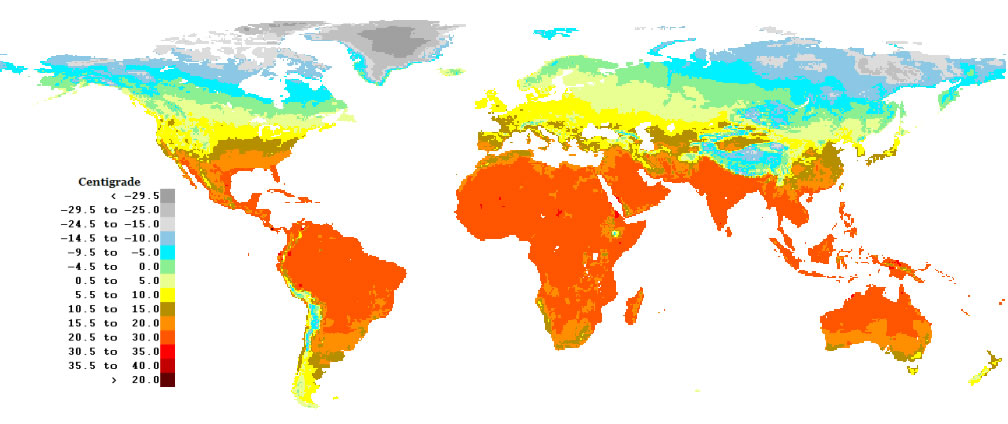
\includegraphics[scale=.45]{./champs/temperatures}
\end{center}



Ce champ de température moyenne est une application ($\Theta_M$) qui associe une température ($\theta_M$) à chaque point ($x,y$) de la surface de la terre.

\begin{align*}
\Theta_M :\ \ \ \ \ \ \ \ \mathbb{R} ^2 \ \  & \rightarrow \ \ \mathbb{R} \\
(x,y) \ \ & \mapsto \ \ \theta_M = \Theta_M(x,y)
\end{align*}

La température dépend du temps (de l'heure, de la date) et des trois dimensions de l'espace,
le champ de température ($\Theta$) est donc une application qui associe une température ($\theta$) à chaque point ($x,y,z,t$) de l'espace-temps.

\begin{align*}
\Theta :\ \ \ \ \ \ \ \ \ \ \ \ \mathbb{R} ^4 \ \  & \rightarrow \ \ \mathbb{R} \\
(x,y,z,t) \ \ & \mapsto \ \ \theta = \Theta(x,y,z,t)
\end{align*}



%%%%%%%%%%%%%%%%%%%%%%%%%%%%%%%%%%%%%%%%%%%%%%%%%%%%%%%%%%%%%%%%%%%%%%%%%%%%

%
\chapter{Champs vectoriels}
%
Un champ vectoriel est une {\it application} qui associe à chaque {\it point de l'espace-temps} un {\it vecteur}.


Dans ce chapitre, nous présentons trois exemples de champs vectoriels.


%%%%%%%%%%%%%%%%%%%%%
\section{Force gravitationnelle}
%%%%%%%%%%%%%%%%%%%%%
%

L'interaction gravitationnelle est une action à distance entre les corps : les corps ayant une masse s'attirent entre eux, la force gravitationnelle modélise l'interaction gravitationnelle. 

La terre exerce sur la lune une action mécanique dont l'effet est d'{\it incurver} sa trajectoire, sans cette action la lune s'éloignerait de la terre.

\setlength{\unitlength}{1cm}
%
\begin{center}
\mbox{%\fbox{
\begin{picture}(17,3)
\put(2,2){\circle{1.52}}
\put(1.6,0.8){Terre}
\thicklines
\put(2,2){\vector(1,0){2.76}}
\put(4.3,2.3){$\overrightarrow{F}_{L/T}$}
\put(15,2){\circle{0.5}}
\put(14.6,1.2){Lune}
\thicklines
\put(15,2){\vector(-1,0){2.76}}
\put(12,2.3){$\overrightarrow{F}_{T/L}$}
\end{picture}}

$\overrightarrow{F_{L/T}}$ : Force gravitationnelle exercée par la lune sur la terre,

 $\overrightarrow{F_{T/L}}$ : Force gravitationnelle exercée par la terre sur la lune.
\end{center}


%%%%%%%%%%%%%%%%%%%%%%%%%%%%%%%%%%%%%%%%%%%%%%%%%%%%%%%%%%%%%%%%%%%%%%%%%%%%

%

%%%%%%%%%%%%%%%%%%%%%
\section{Champ électrique et potentiel scalaire}
%%%%%%%%%%%%%%%%%%%%%
%
Le champ électrique créé par une particule chargé s'étend dans l'espace à 3 dimensions. Il est possible, afin de simplifier les schéma de se limiter à 2 dimensions.

Le champ électrique créé par une particule chargée est radial et son amplitude décroit avec la distance à la particule.

\begin{center}
\tikzstyle{fleche}=[->,line width=1pt]
\begin{tikzpicture}
  \begin{scope}[xshift=0 cm,yshift=0 cm, scale = 1.6]%
\foreach \t in {60,120, ...,360}
\draw [fleche] (\t:1) -- (\t:2.8);
\foreach \t in {30,90, ...,360}
\draw [fleche] (\t:2) -- (\t:2.45);
\foreach \t in {15,45,-15,-45}
\draw [fleche] (\t:3) -- (\t:3.2);
\foreach \t in {15,45,-15,-45}
\draw [fleche] (\t+180:3) -- (\t+180:3.2);
\draw [fill=red] (0,0) circle(0.1) node [above right] {$Q_1$};
  \end{scope}
\end{tikzpicture}
\end{center}


Comme le champ de pente dérive d'un champ scalaire (le champ d'altitude), le champs electrique dérive d'un champ scalaire. On l'appelle le potentiel électrique. On représente ci-dessous les lignes de même potentiel (équi-potentiel) du potentiel électrique créé par une particule chargée.

\begin{center}
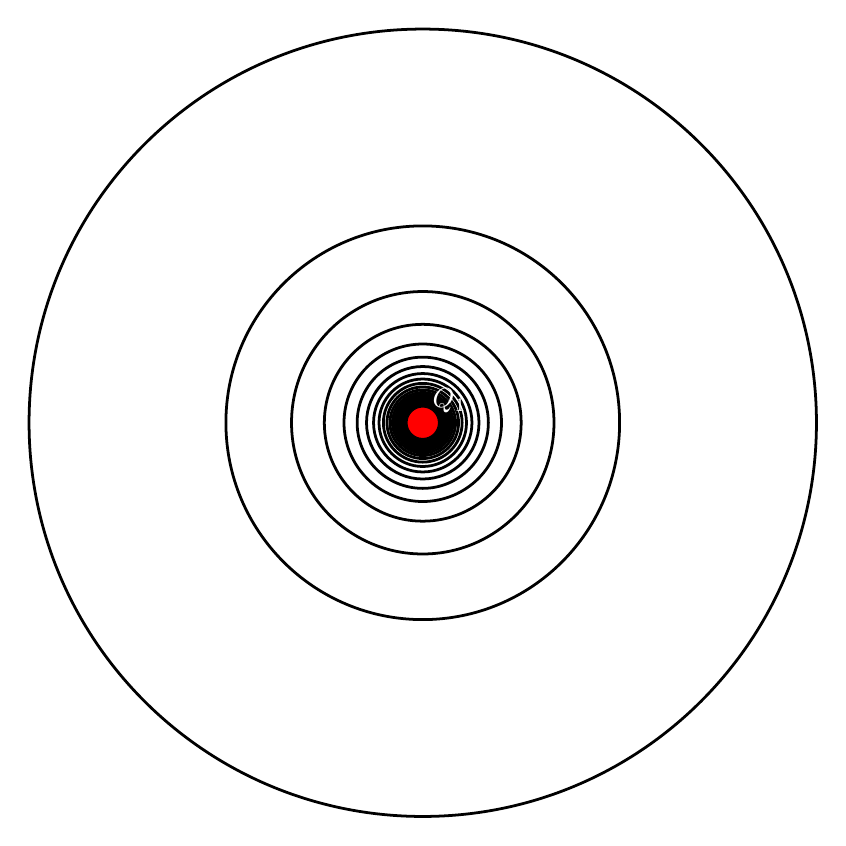
\begin{tikzpicture}
  \begin{scope}[xshift=0 cm,yshift=0 cm, scale = 1]%
\foreach \t in {1,2, ...,30}
\draw [line width=1pt] (0,0) circle (5/\t) ;

\draw [fill=red] (0,0) circle(0.2) node [above right,text=white] {$Q_1$};
  \end{scope}
\end{tikzpicture}
\end{center}

En 3 dimensions, les points de même potentiel sont des surfaces. Les surfaces équi-potentiel du potentiel créé par une particule chargée sont des sphères.

%%%%%%%%%%%%%%%%%%%%%%%%%%%%%%%%%%%%%%%%%%%%%%%%%%%%%%%%%%%%%%%%%%%%%%%%%%%%

%

%%%%%%%%%%%%%%%%%%%%%
\section{Force magnétique}
%%%%%%%%%%%%%%%%%%%%%
%

La force magnétique est la force qui s'exerce entre les \textbf{\textit {aimants}}.
Les aimants sont des matériaux possédant des propriétés magnétiques.
Certain métaux peuvent être aimantés par la proximité d'un aimant.

\subsection{Pôles magnétiques}

Un aimants est toujours {\it orienté}, il possède un pôle dit \textbf{\textit {nord}} et un pôle
dit \textbf{\textit {sud}}.


\subsection{Action magnétique}

La force magnétique entre deux aimants, est attractive et répulsive, elle exerce un {\it couple} :
entre deux aimants, les pôles opposés s'attirent, les pôles identiques se repoussent. 

Ci-dessous, deux aimants sont schématisés, les pôles nord en rouge et les pôles sud en bleu. On ne représente que les forces que l'aimant 2 exerce sur l'aimant 1.

\begin{center}
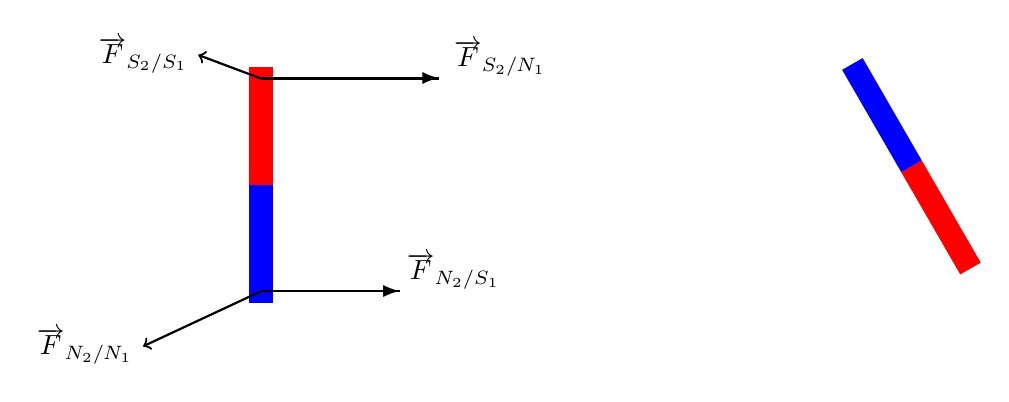
\begin{tikzpicture}[scale=1]
\fill [blue] (0,0) rectangle (0.3,1.5);
\fill [red] (0,1.5) rectangle (0.3,3);
\begin{scope}[rotate=30,yshift=-4.2cm]%
\fill [red] (8,0) rectangle (8.3,1.5);
\fill [blue] (8,1.5) rectangle (8.3,3);
\end{scope}
\thicklines
\put(0.15,0.15){\vector(1,0){1.76}}
\put(2,0.3){$\overrightarrow{F}_{N_2/S_1}$}

\put(0.15,2.85){\vector(1,0){2.26}}
\put(2.6,3){$\overrightarrow{F}_{S_2/N_1}$}

\draw [thick] [->] ((0.15,(0.15) --++(-1.5,-0.7) node [left] {$\overrightarrow{F}_{N_2/N_1}$};

\draw [thick] [->] ((0.15,(2.85) --++(-0.8,0.3) node [left] {$\overrightarrow{F}_{S_2/S_1}$};

%\put(0.15,0.15){\vector(-1,-1){0.5}}
%\put(4.3,2.3){$\overrightarrow{F}_{L/T}$}
\end{tikzpicture}
\end{center}
%%%%%%%%%%%%%%%%%%%%%%%%%%%%%%%%%%%%%%%%%%%%%%%%%%%%%%%%%%%%%%%%%%%%%%%%%%%%

%

